% Source-page vector redraw from 2005 Spring Beijing Science, printed p. 213, Q16.
% Schematic perspective only. Dashed segments are the source's obscured original triangle edges.
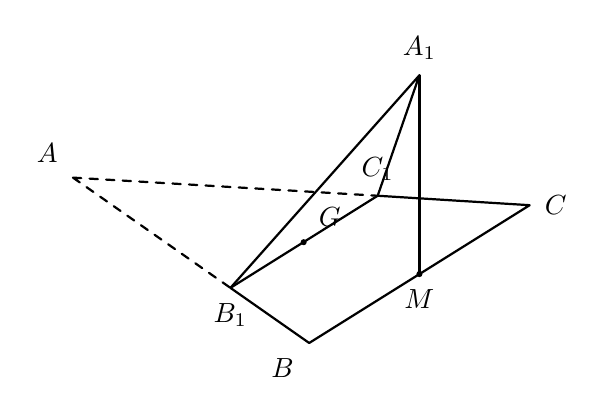
\begin{tikzpicture}[line cap=round, line join=round, scale=1.0]
\coordinate (A) at (-2,.90); \coordinate (B) at (1,-1.20); \coordinate (C) at (3.8,.55);
\coordinate (B1) at (0,-.50); \coordinate (C1) at (1.87,.67);
\coordinate (G) at (.93,.08); \coordinate (M) at (2.4,-.325); \coordinate (A1) at (2.4,2.2);
% Original triangle portions, folded triangle, and crease
\draw[dashed, thick] (A)--(B1) (A)--(C1);
\draw[thick] (B1)--(B)--(C)--(C1)--cycle;
\draw[thick] (A1)--(B1) (A1)--(C1);
% Median/projection line and named points on the crease/base
\draw[thick] (A1)--(M);
\fill (G) circle (1.1pt) (M) circle (1.1pt);
\node[above left=2pt] at (A) {$A$};
\node[below left=2pt] at (B) {$B$};
\node[right=2pt] at (C) {$C$};
\node[below=2pt] at (B1) {$B_1$};
\node[above=2pt] at (C1) {$C_1$};
\node[above right=2pt] at (G) {$G$};
\node[above=2pt] at (A1) {$A_1$};
\node[below=2pt] at (M) {$M$};
\end{tikzpicture}
